\documentclass[SKL-MASTER.tex]{subfiles}
\begin{document}
\LARGE
\noindent\textbf{Evaluating Models with ROC Curves}
\begin{itemize}
\item Receiving Operating Characteristic, or ROC, is a visual way for inspecting the performance of a binary classification algorithm. 
\item In particular, it's comparing the rate at which your classifier is making correct predictions (\textit{True Positives} or TP) and the rate at which your classifier is making false alarms (\textit{False Positives} or FP). 
\item When talking about True Positive Rate (TPR) or False Positive Rate (FPR) we're referring to the definitions below:
\end{itemize}

\[ \mbox{TPR}= \frac{\mbox{True Positives}}{\mbox{True Positives + False Negatives} } \]
\[ \mbox{FPR}=\frac{\mbox{False Positives}}{\mbox{False Positives + True Negatives} }\]

\noindent \textit{\textbf{Remark} True Positives Rates and True Negatives Rates referred to as Sensitivity and Specificity.}
%\begin{itemize}
% \item You might have heard of.
%\item  No matter what you call it, the big point here is we're measuring the trade off between the rate at which you can correctly predict something, with the rate at which you make an embarrassing blunder and predict something that doesn't happen.
%\end{itemize}
%-------------------------------------------------------------------------- %
\newpage
\noindent\textbf{Background } \\
\begin{itemize}
\item ROC curves were first used during WWII to analyze radar effectiveness. 
\item In the early days of radar, it was sometimes hard to tell a large bird from an incoming airplane. 
\item The British Ministry of Defence pioneered using ROC curves to optimize the way that they could rely to radar for detect approaching Luftwaffe airplanes.
\end{itemize}

%--------------------------------------------------------------------------- %


\newpage
\noindent \textbf{Scenarios: Guessing at Random}
\begin{itemize}
\item The first example is the simplest: a diagonal line. 
\item A diagonal line indicates that the classifier is just making completely random guesses.
\item Since your classifier is only going to be correct 50\% of the time, it stands to reason that your TPR and FPR will also be equal.
\end{itemize}


\begin{figure}[h!]
\centering
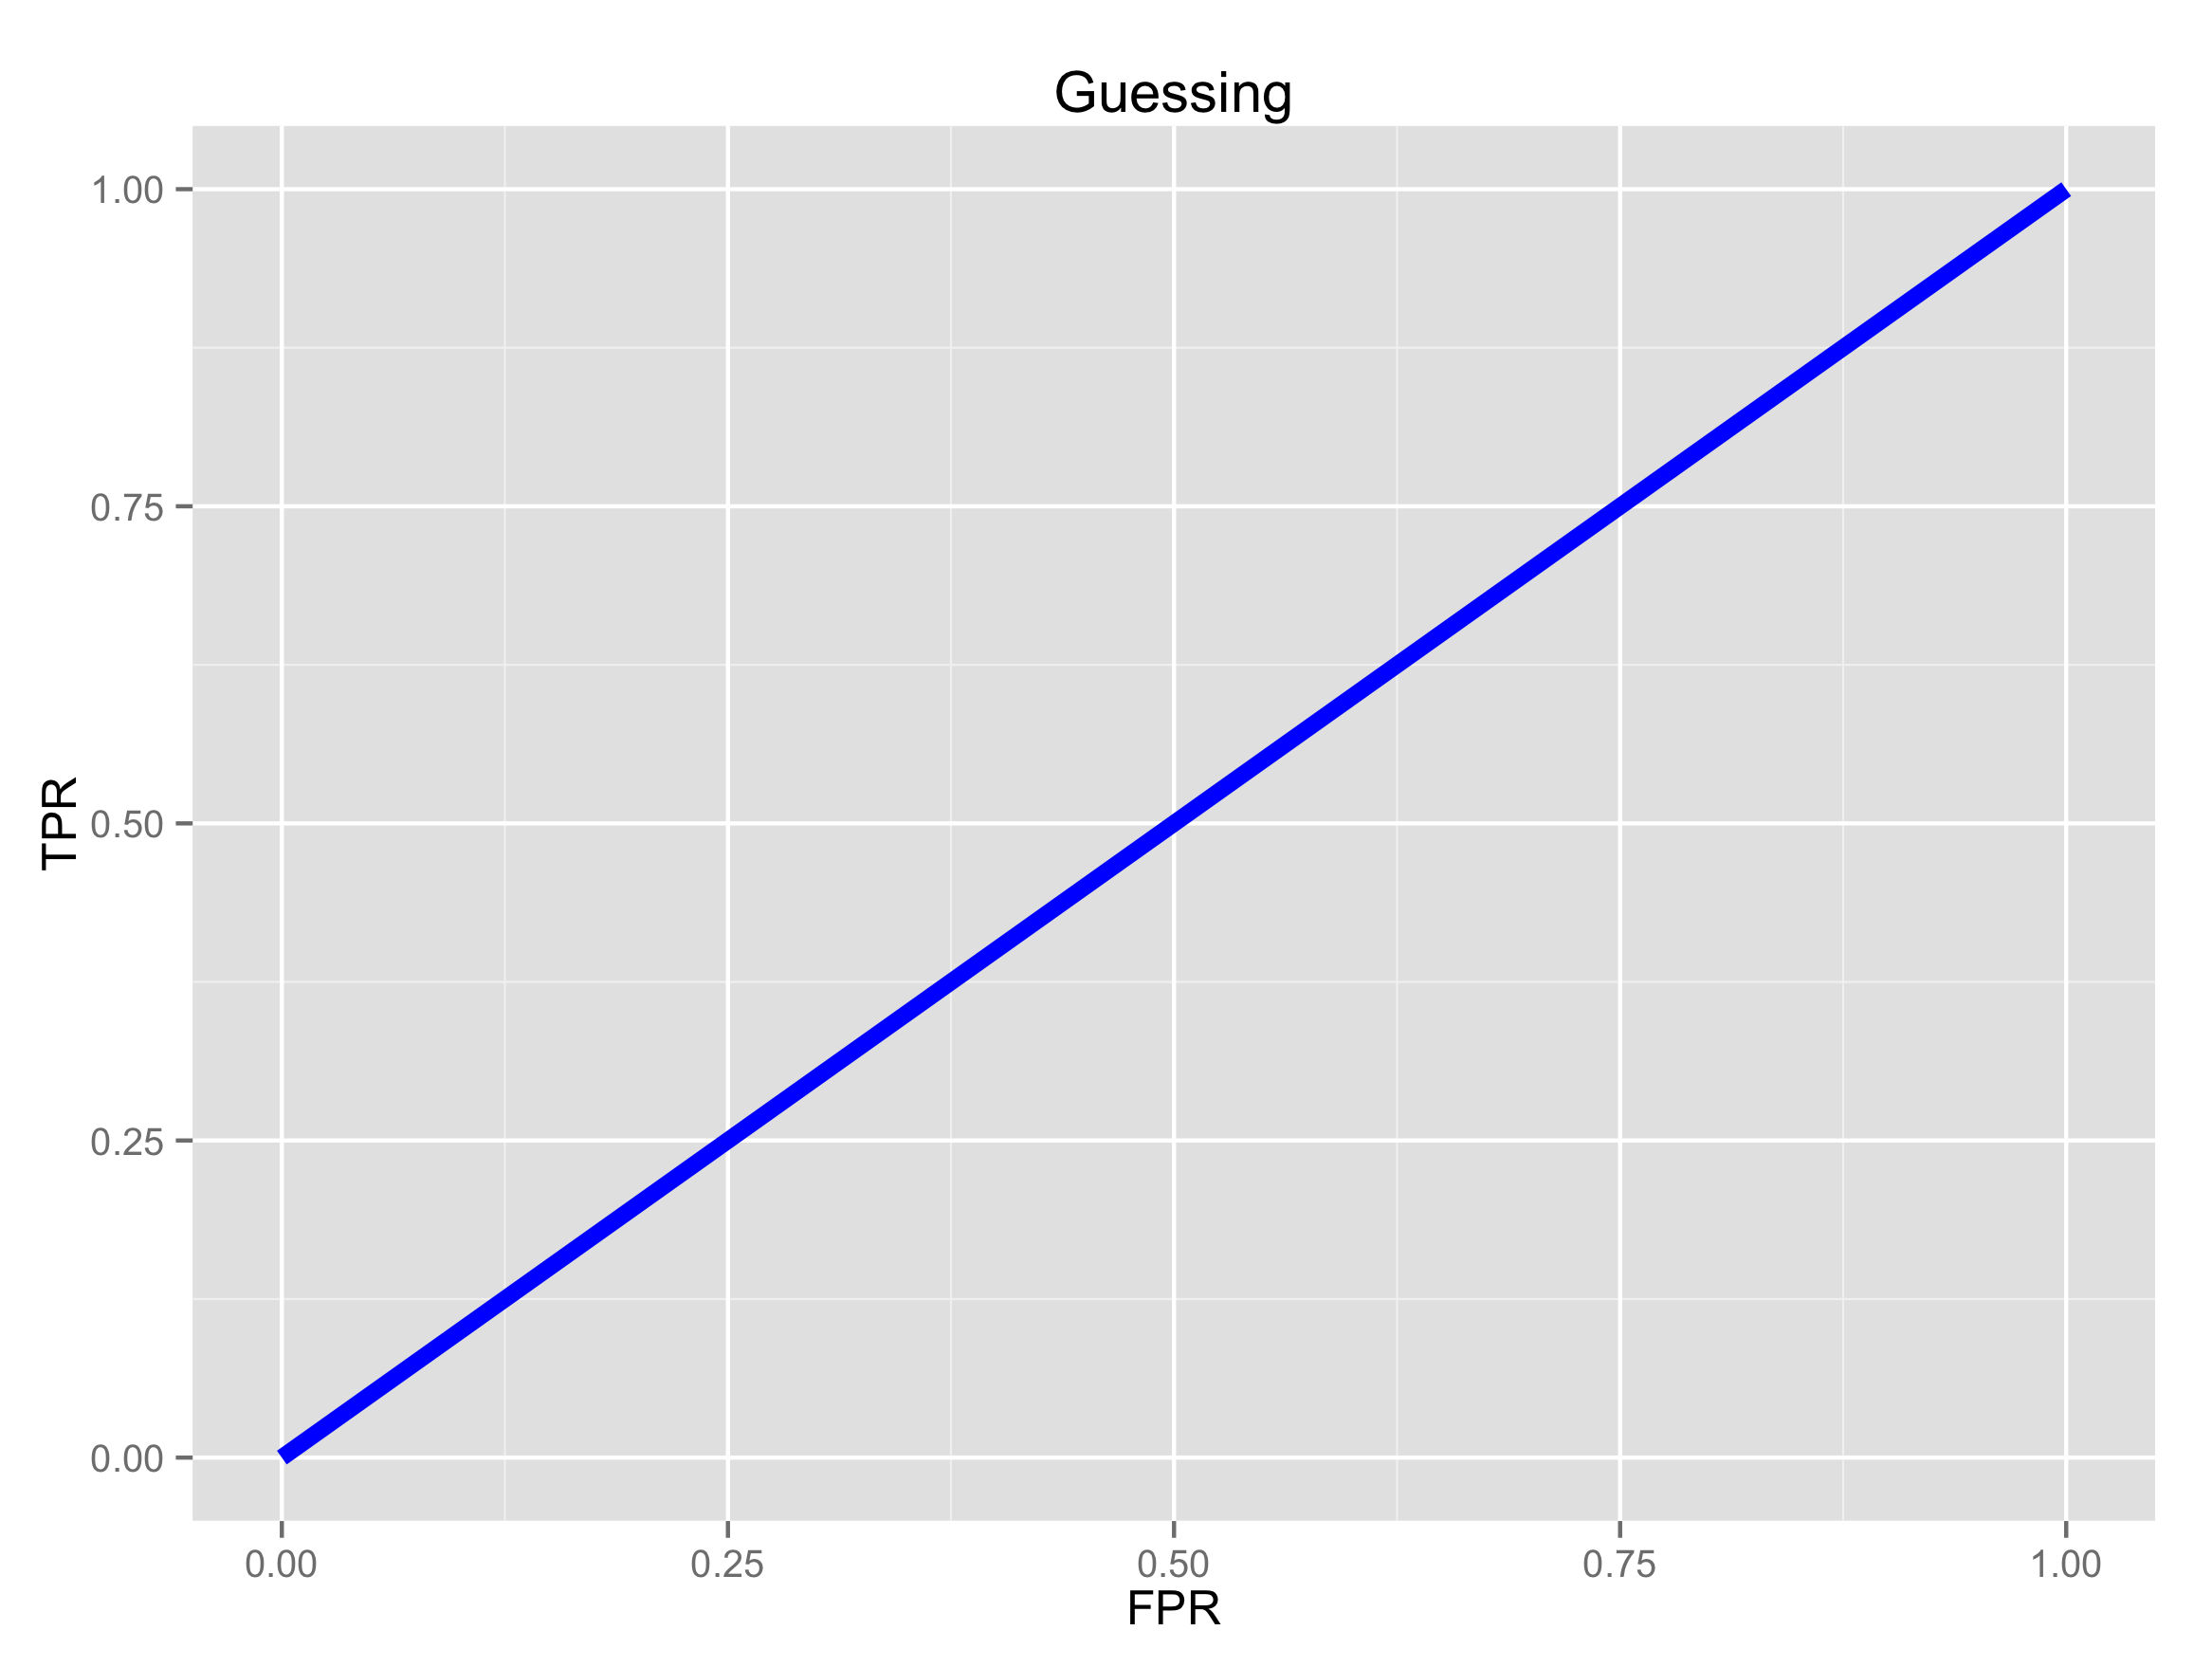
\includegraphics[width=0.7\linewidth]{images/roc-guessing}
\end{figure}
\noindent Often, ROC charts will include the random ROC curve to provide the user with a benchmark for what a naive classifier would do.\\  Any curves above the line are better than guessing, while those below the line, you would be better off guessing.
\\
\noindent \textit{For review: The Area Under the Curve (AUC)  is 0.500.} 
\newpage
\noindent \textbf{A Perfect Classifier}
\begin{itemize}
\item 
A perfect classifier will yield a perfect trade-off between TPR and FPR (meaning you'll have a TPR of 1 and an FPR of 0).
\item In that case, your ROC curve looks something like this.
\end{itemize}

\begin{figure}[h!]
\centering
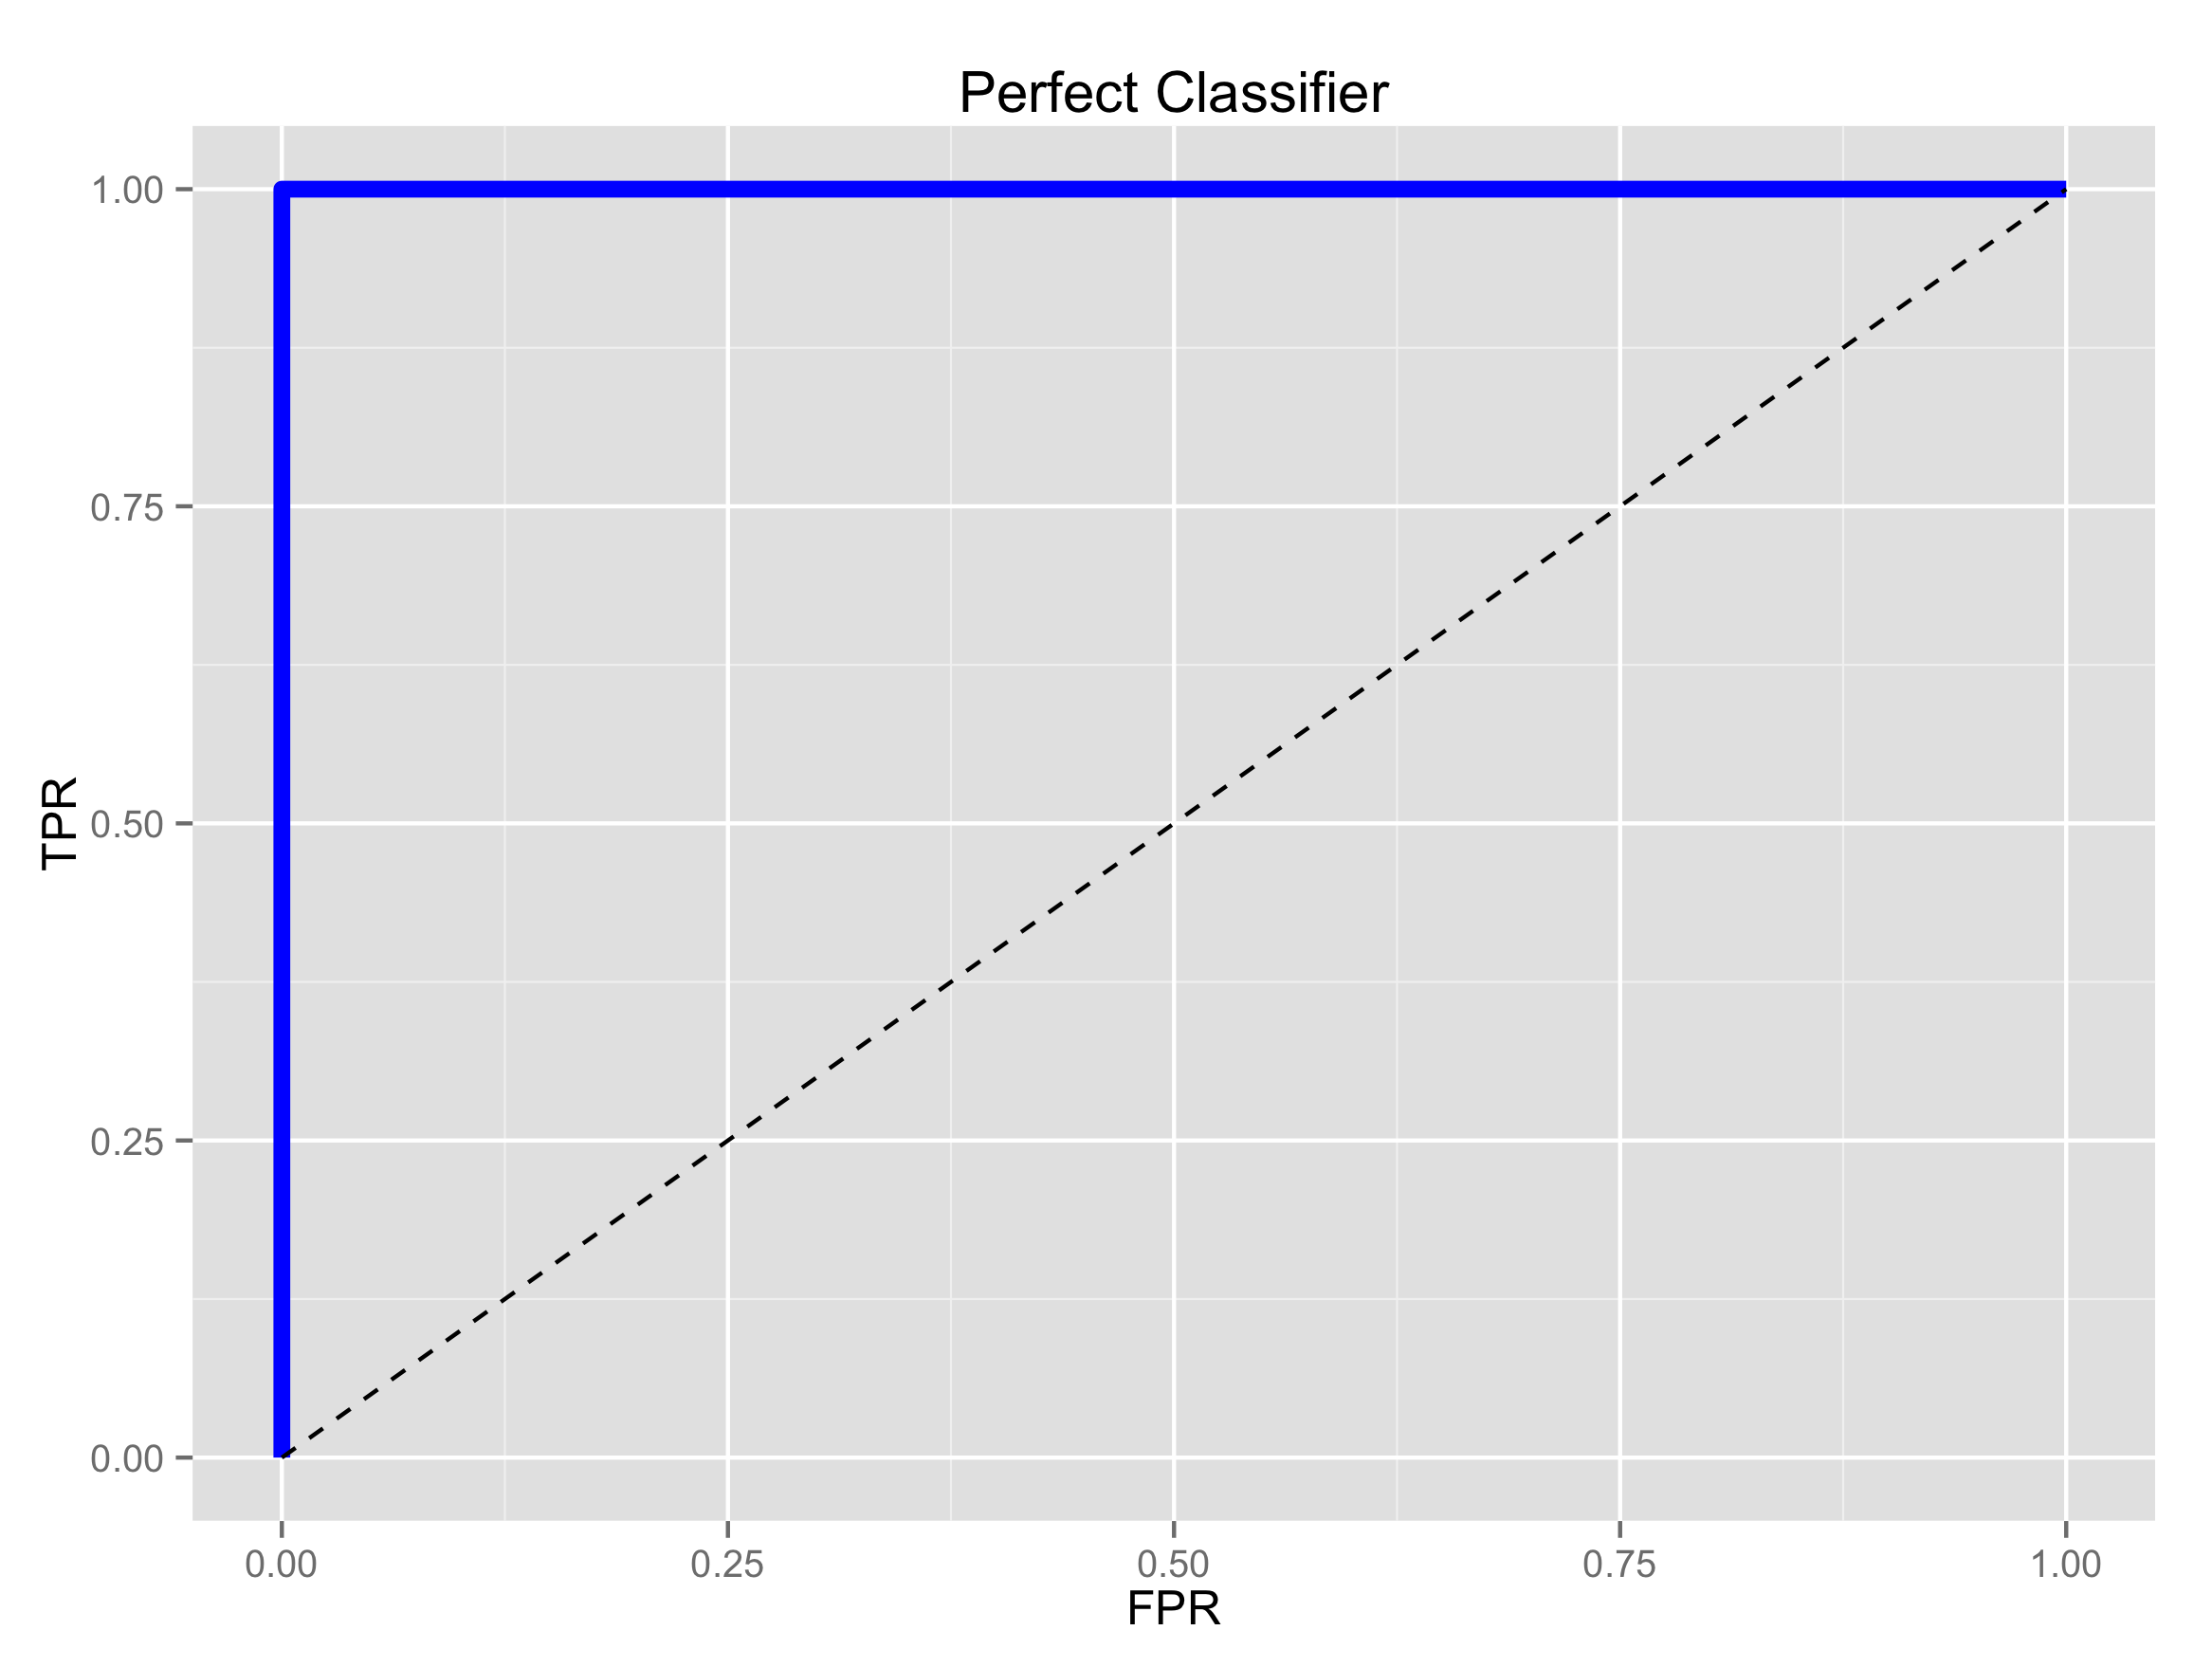
\includegraphics[width=0.7\linewidth]{images/roc-perfect}
\end{figure}
\begin{framed}
\noindent \textbf{Important:} The better your classifier, the more closer the curve will be to the top left corner.
\end{framed}
\noindent \textit{For review: Note the "random curve" is included as a benchmark as a dotted line.\\ 
The Area Under the Curve (AUC) is 1.}
\newpage
\noindent \textbf{Worse than guessing}\\

\noindent A bad classifier (i.e. something that's worse than guessing) will appear mostly below the random line. 

\begin{figure}[h!]
\centering
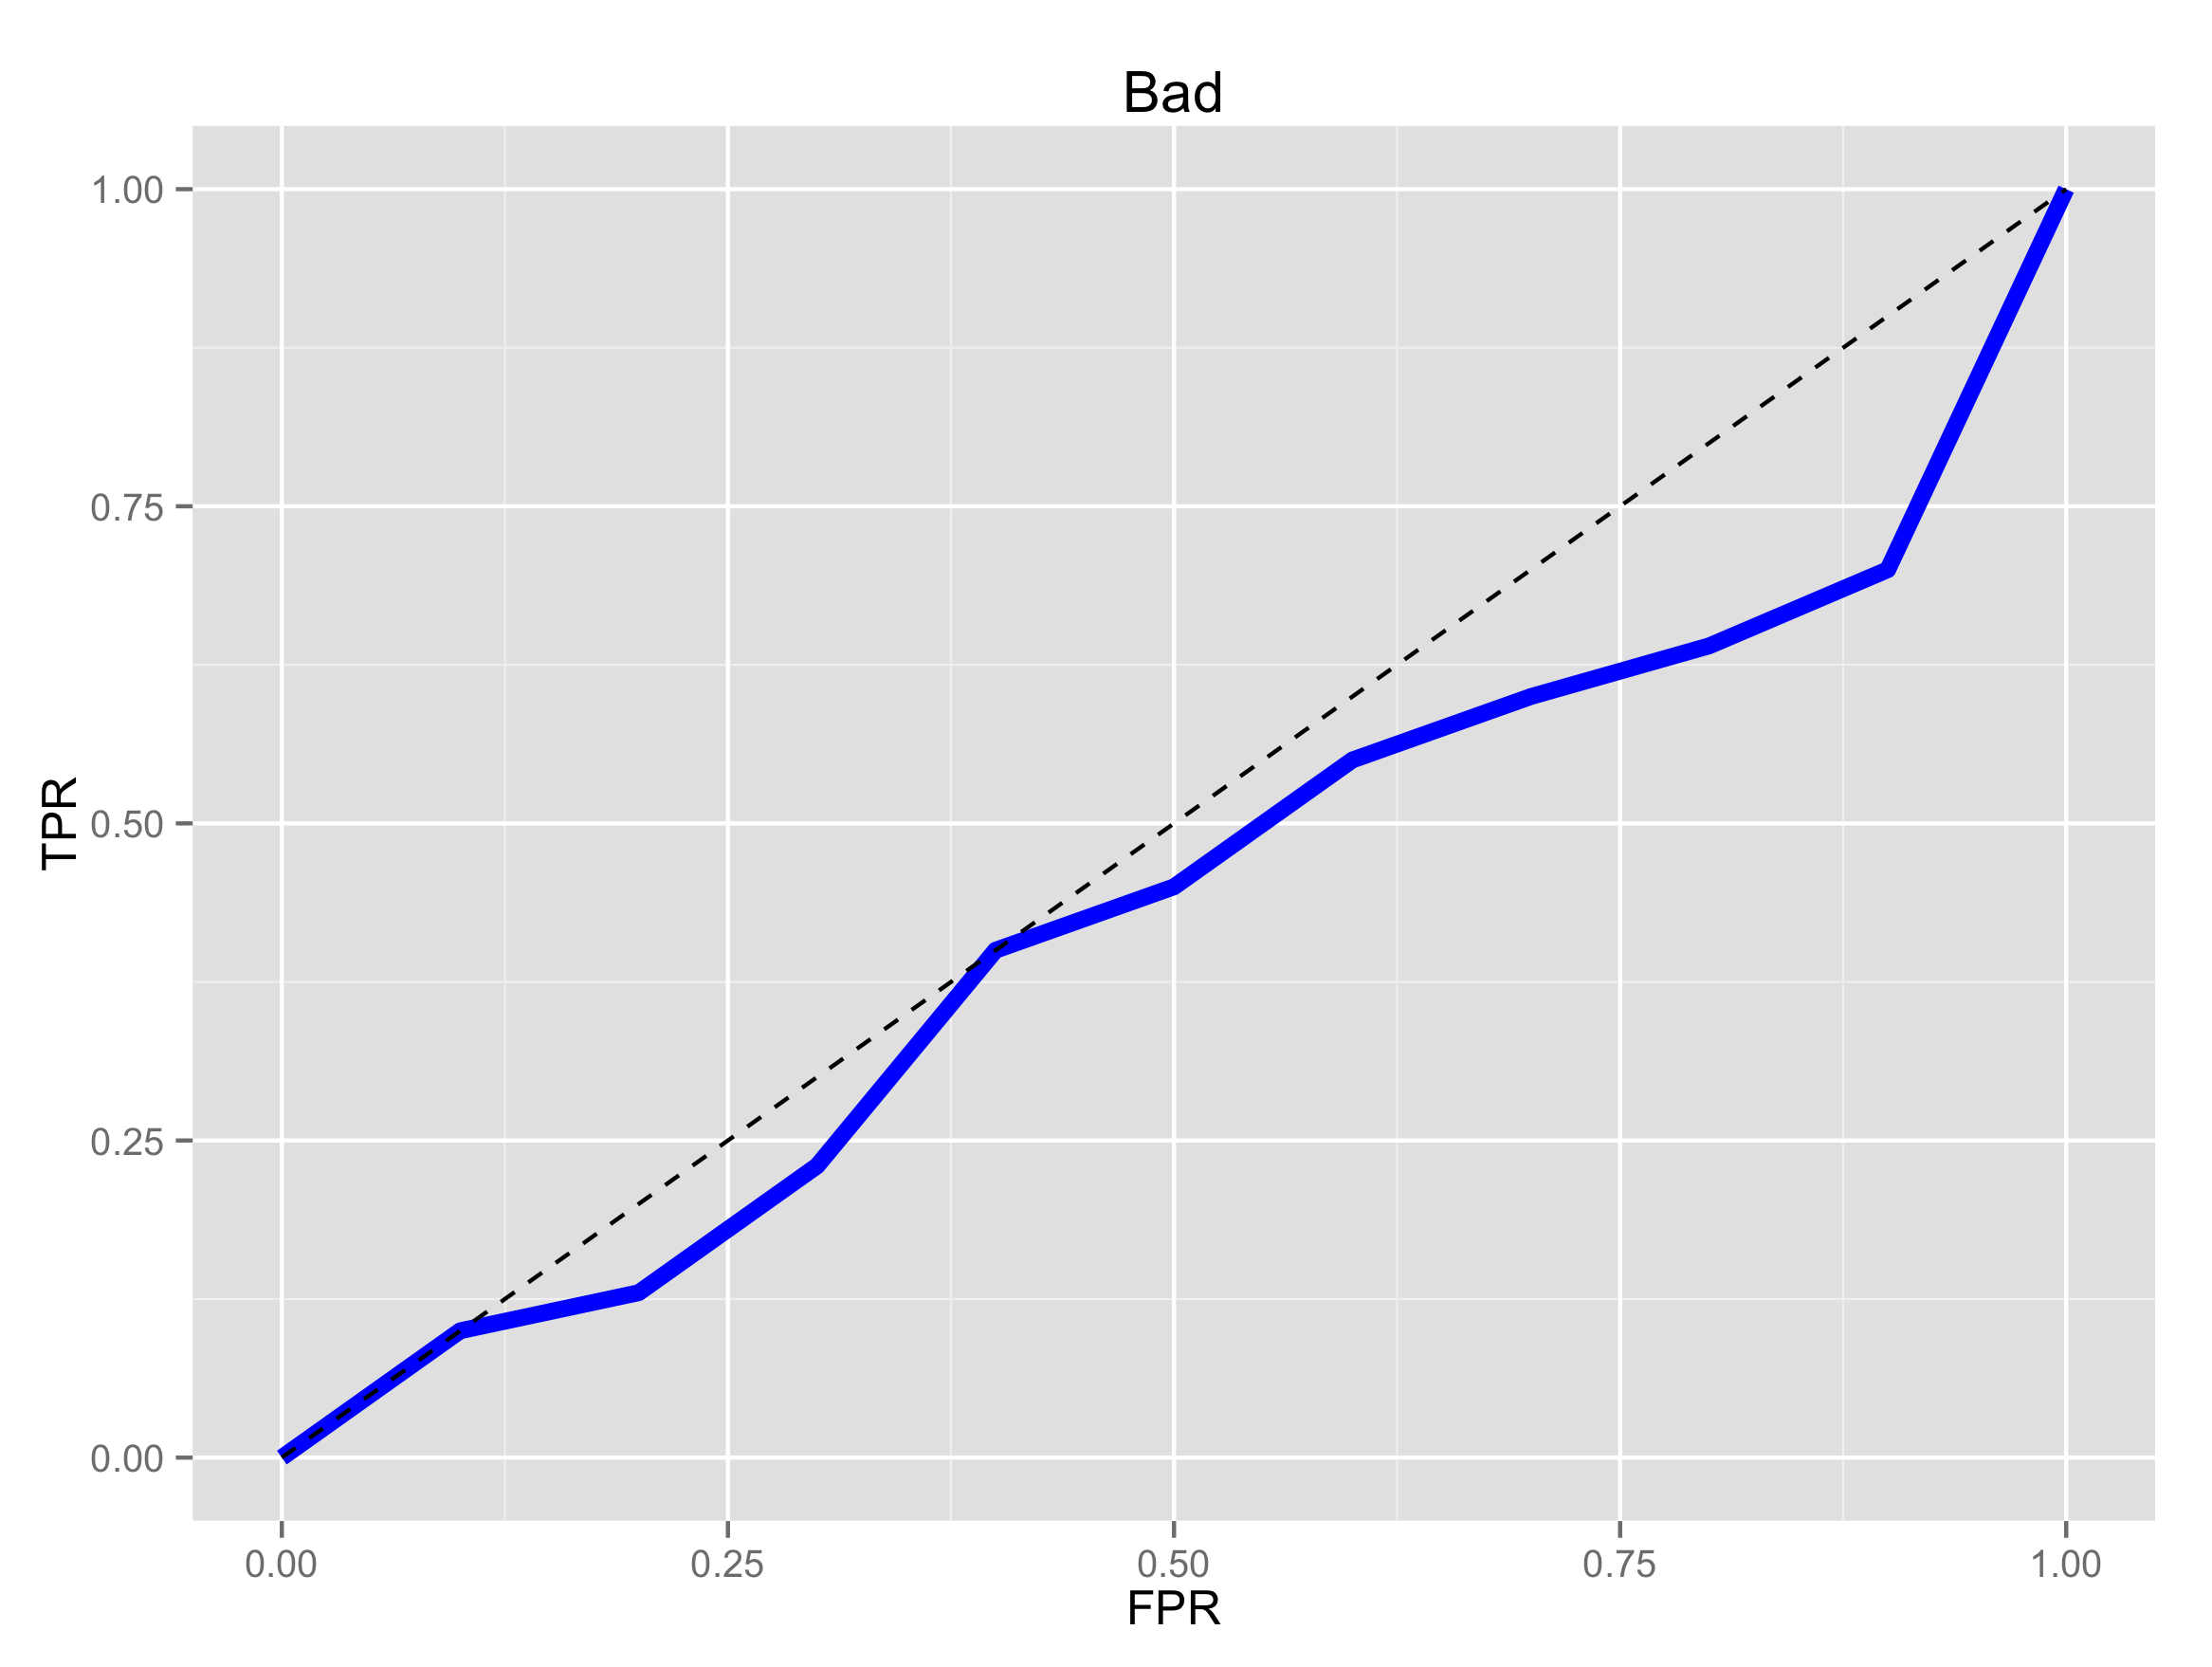
\includegraphics[width=0.9\linewidth]{images/roc-bad}
\end{figure}

\noindent There have been several instances of a ``prediction system" underperforming "guessing at random".
\newpage
\noindent \textbf{Better than guessing}



\noindent A much more interesting activity is attempting to decipher the difference between an "OK" and a "Good" classifier. The chart below shows an example of a very mediocre classifier. It is still better than guess at random though.

\begin{figure}[h!]
\centering
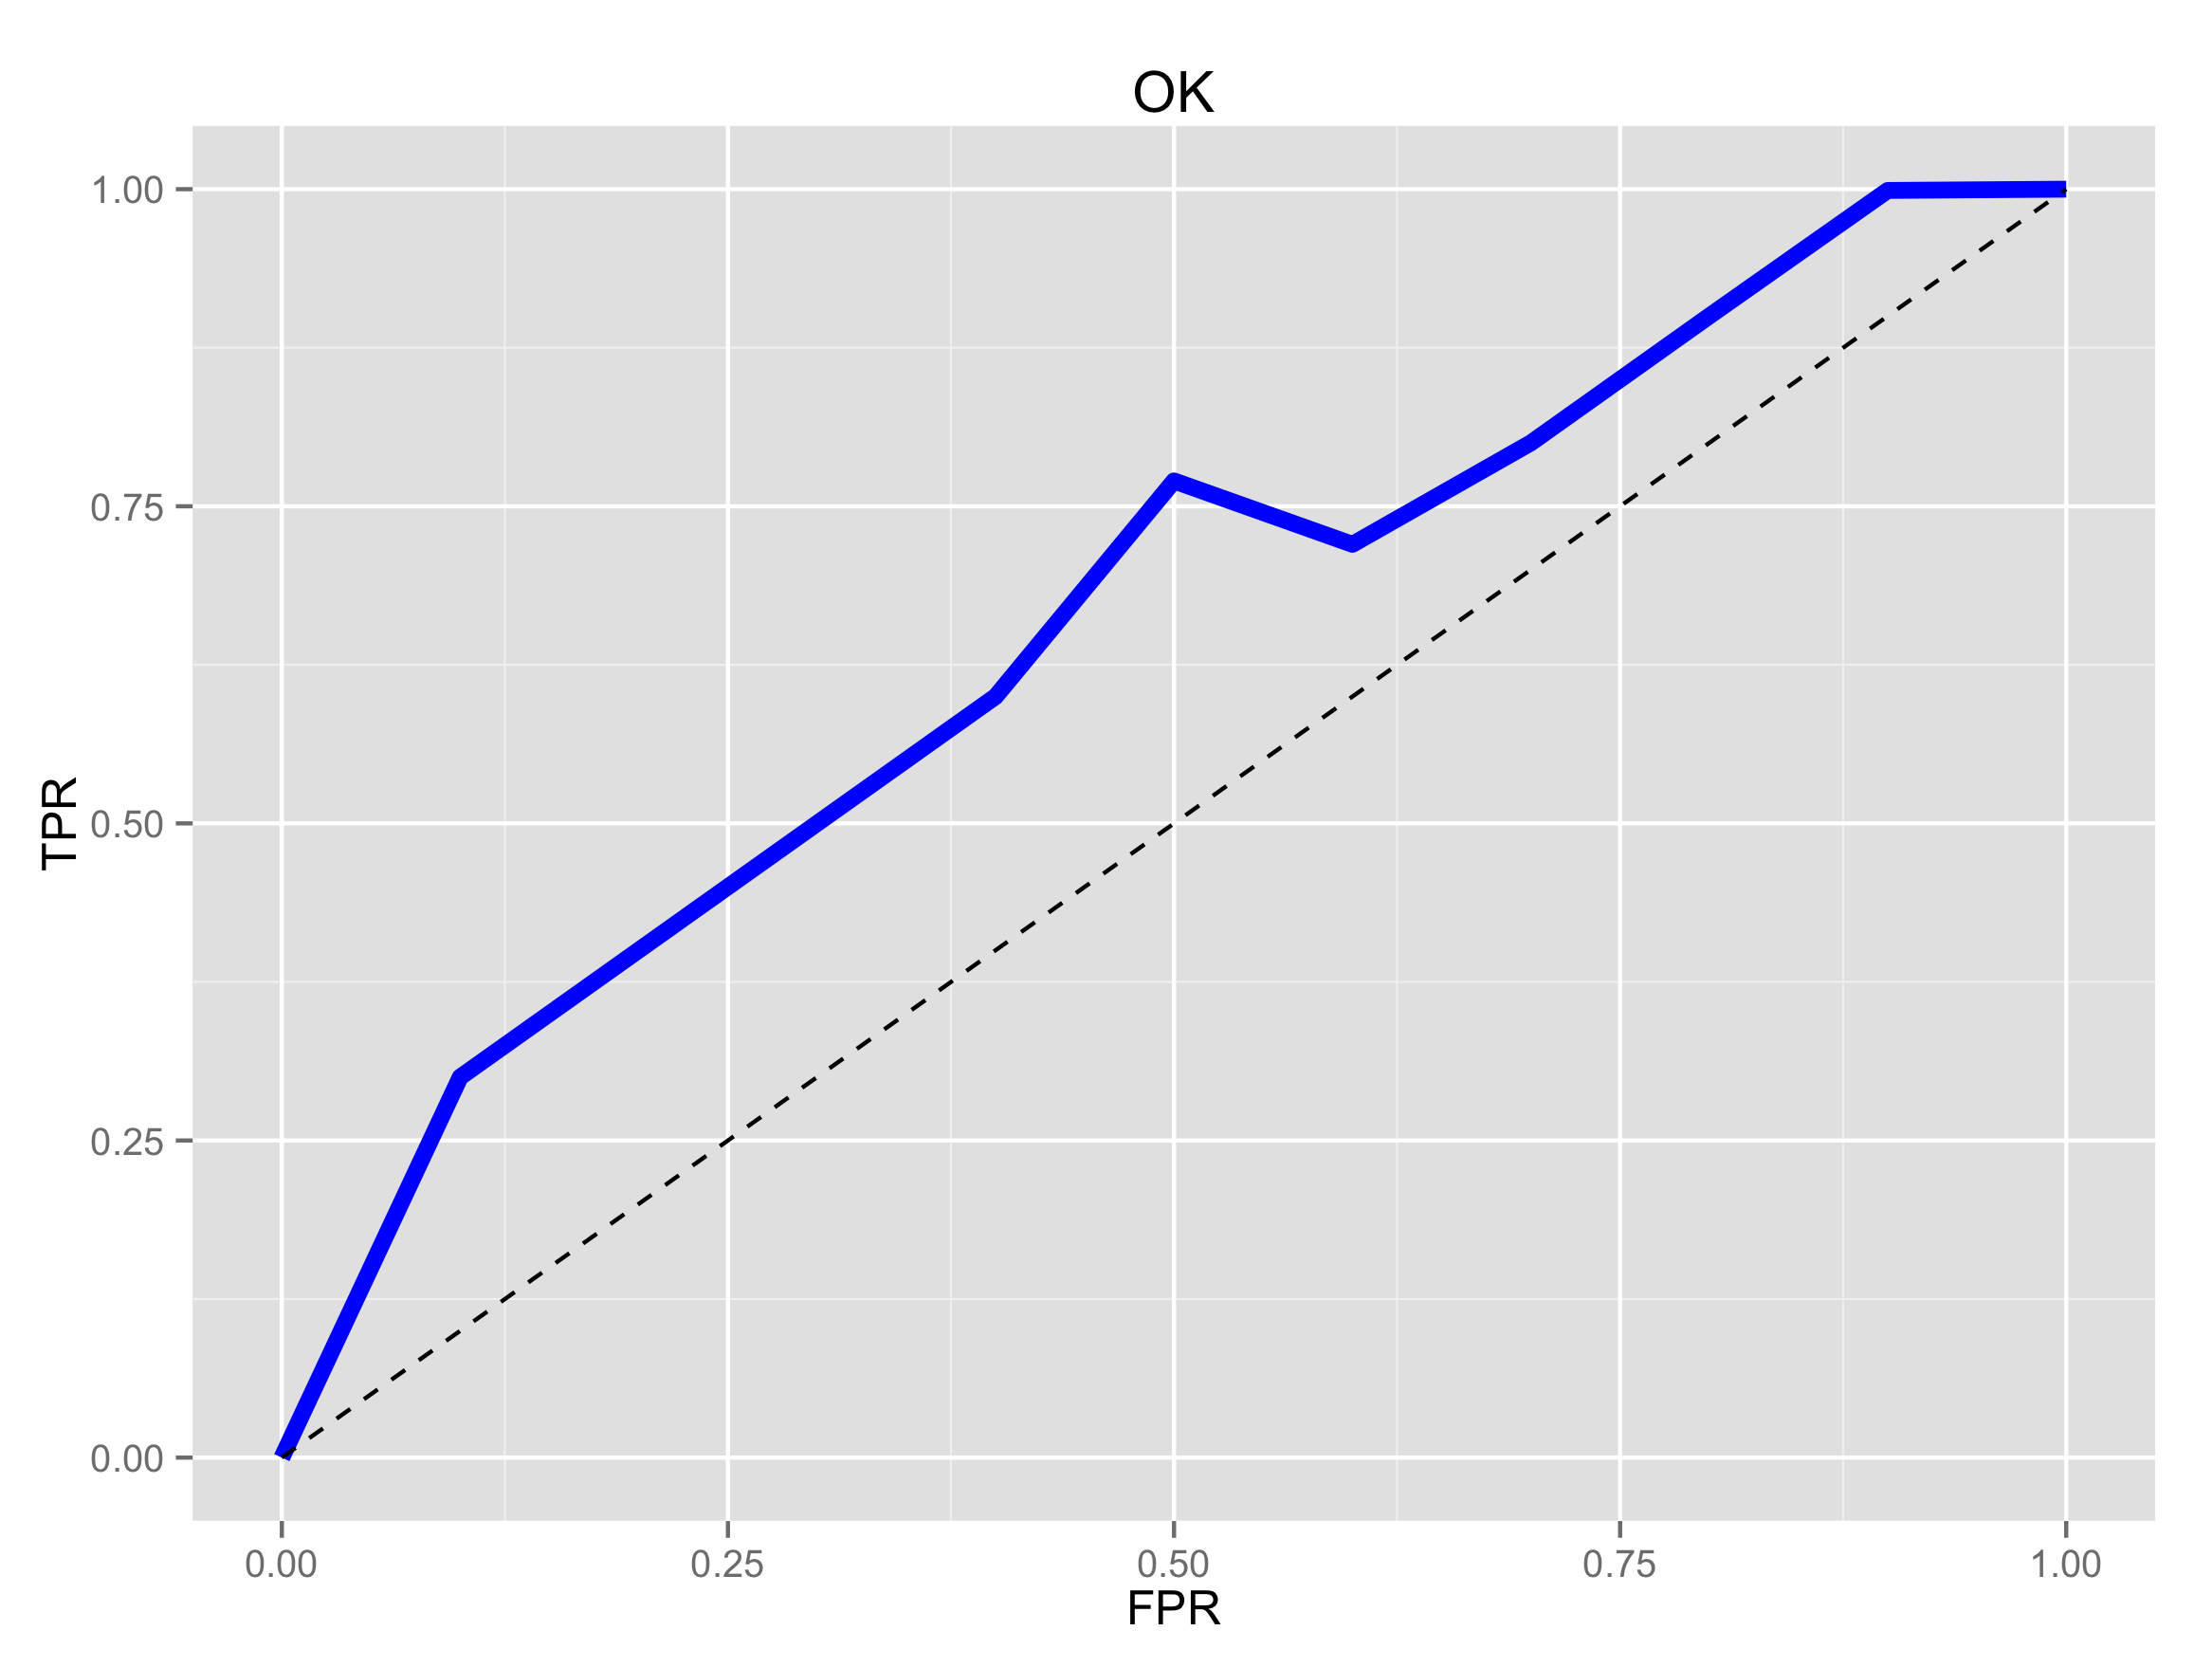
\includegraphics[width=0.9\linewidth]{images/roc-ok}
\end{figure}
%
%
% Context is everything of course, but there's not much lift here. In addition, be very wary of lines that dip or are very geometric looking. I've found that in practice, this can mean that there's an irregularity with your data, or you're making a very bad assumption in your model.


\newpage
\noindent \textbf{Reasonably Good}

%Ahh this is looking a little better. Below you can see a nice "hump shaped" (it's a technical term) curve that's continually increasing. It sort of looks like it's being yanked up into that top left (the perfect) spot of the chart.

In practice, most decent classification systems have a ROC curve like this.  Recall that better a prediction system is , the closer it is to the top left.
\begin{figure}[h!]
\centering
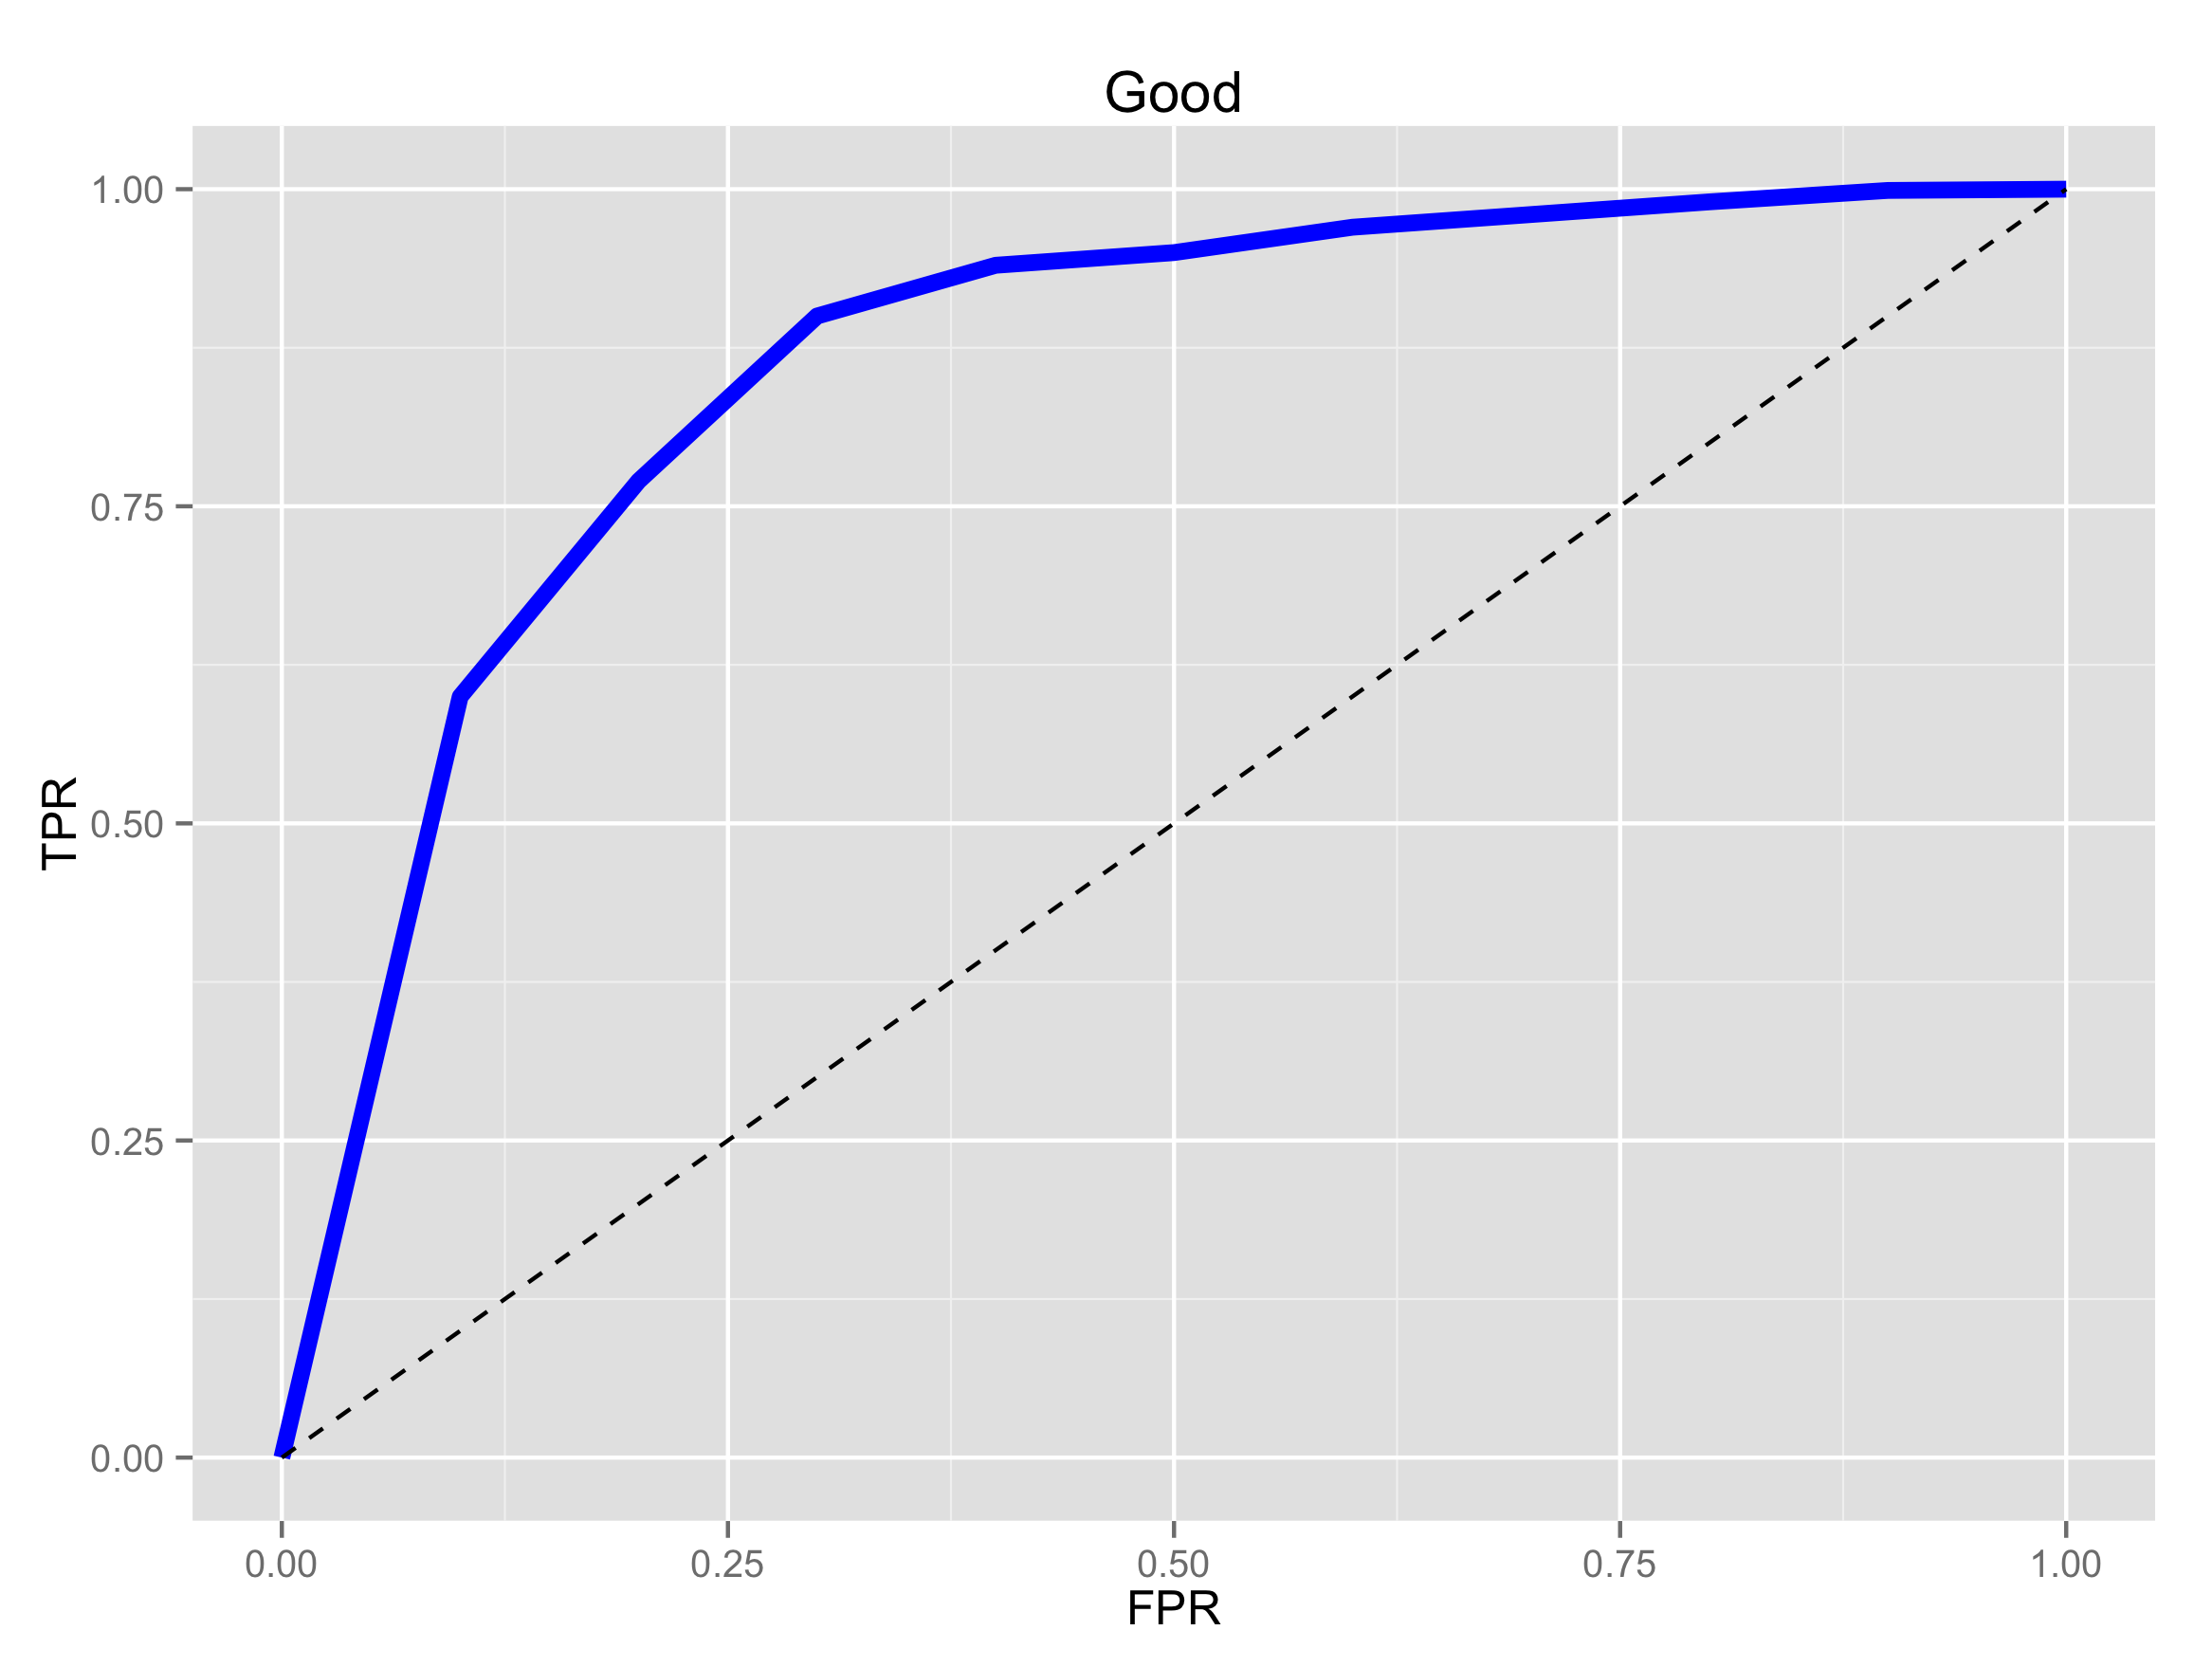
\includegraphics[width=0.9\linewidth]{images/roc-pretty-good}

\end{figure}

%%============================================================================== %
\newpage
\noindent \textbf{Area under the curve (AUC)}

\noindent There is an aggregate metric to determine how good the prediction system is:  AUC or Area Under the Curve. 

\noindent The AUC is the amount of space underneath the ROC curve

\begin{itemize}
\item AUC = 0 :  Perfectly Bad
\item AUC $< 0.5$ : Worse than guessing at random 
\item AUC = 0.5 : same as guessing at random
\item AUC $> 0.5$ : Good. better than guessing at random
\item AUC = 1 : Perfectly Good
\end{itemize}
%
%
%
\noindent Comparing AUC values is useful when comparing different models, as we can select the model with the high AUC value, rather than just look at the curves.
\end{document}


